\documentclass[10pt,a4paper]{report}

% Packages
\usepackage[utf8]{inputenc}
\usepackage[francais]{babel}
\usepackage{hyperref}
\usepackage{color}
\usepackage{colortbl}
\usepackage{multirow}
\usepackage{verbatim}
\usepackage{moreverb}
\usepackage{amsmath}
\usepackage{amsfonts}
\usepackage{amssymb}
\usepackage{wrapfig}
\usepackage{graphicx}
%\usepackage[T1]{fontenc}
%\usepackage{lmodern}
\usepackage[footnote]{acronym}
\usepackage{array}
\usepackage{dirtree}

% Links
\definecolor{couleur_liens}{rgb}{0, 0, 0.5}

% Acronyms
\acrodef{svn}[svn]{Subversion}

% Tables
\definecolor{table_header_color}{rgb}{1,1,1}%{rgb}{0.85, 0.95, 1}
\newcolumntype{C}[1]{>{\centering\let\newline\\\arraybackslash\hspace{0pt}}m{#1}}

% Settings..
\author{LAFON Sylvain pour Manzalab}
\title{Utilisation du gestionnaire de version :\\Git}
\hypersetup{
    %bookmarks=true, % show bookmarks bar?
    unicode=false, % non-Latin characters in Acrobat’s bookmarks
    pdftoolbar=true, % show Acrobat’s toolbar?
    pdfmenubar=true, % show Acrobat’s menu?
    pdffitwindow=false, % window fit to page when opened
    pdfstartview={FitH}, % fits the width of the page to the window
    pdftitle={Git Tuto}, % title
    pdfauthor={LAFON Sylvain pour Manzalab}, % author
    pdfsubject={Tutoriel sur git}, % subject of the document
    pdfcreator={Latex}, % creator of the document
    pdfproducer={Texmaker}, % producer of the document
    pdfkeywords={git} {tuto}, % list of keywords
    pdfnewwindow=true, % links in new window
    colorlinks=true, % false: boxed links; true: colored links
    %hidelinks,
    urlcolor=couleur_liens, % color of external links
    linkcolor=black, % color of internal links
    citecolor=green, % color of links to bibliography
    filecolor=magenta, % color of file links
}

\begin{document}
	\maketitle
	% Preface
\section*{Preface}
Voici un document crée à partir de mes connaissances sur git et de quelques sources issues d'Internet. Je ne vais PAS détailler les commandes que j'utilise souvent ni même les fenêtres qui apparaîtrons dans Tortoise Git, une interface que nous allons utiliser.\\

Si vous voulez maîtriser git et connaître toutes ses commandes de fond en comble, vous devrez utiliser \href{https://www.kernel.org/pub/software/scm/git/docs/}{le manuel} ou bien internet.\\

La plupart des commandes git ont l'option --help :
\begin{verbatim}
$ git <commande> --help 
$ git help <commande>
$ man git-<commande>
\end{verbatim}

Si vous souhaitez connaître les options d'une fenêtre en particulier, le mieux reste de trouver quelle commande la fenêtre appellera et de regarder ses options sur internet.\\

Ce tutoriel est certes technique mais part de zéro : n'importe qui devrait pouvoir le lire. Si un passage n'est pas clair, je reste disponible à l'adresse sylvain.lafon.91@gmail.com : je vous expliquerai ledit passage et modifierai le document afin de retirer les ambiguïtés et autres passages obscurs.\\

Le tutoriel officiel de git se trouve dans le manuel :
\begin{itemize}
\item Première partie : \href{https://www.kernel.org/pub/software/scm/git/docs/gittutorial.html}{gittutorial (7)}
\item Seconde partie : \href{https://www.kernel.org/pub/software/scm/git/docs/gittutorial-2.html}{gitutorial-2 (7)}
\item \href{https://www.kernel.org/pub/software/scm/git/docs/user-manual.html}{Manuel complet}
\item \href{https://www.kernel.org/pub/software/scm/git/docs/everyday.html}{Commandes de base}\\
\end{itemize}

Ce livre peut également vous être très utile : \href{https://git-scm.com/book/fr/v2}{Pro Git} aussi disponible dans sa \href{https://progit2.s3.amazonaws.com/fr/2016-03-05-4c838/progit-fr.1062.pdf}{version PDF}

	\newpage
\section*{Versions}

%
% +---------+----------+-----------------------------------------+
% | Version | Date | Description |
% +---------+----------+-----------------------------------------+
%

\begin{tabular}{|c|c|C{7.5cm}|}
\hline
\rowcolor{table_header_color}
\begin{bf}Version\end{bf} & \begin{bf}Date\end{bf} & \begin{bf}Description\end{bf} \\
\hline
v1.0 & 16.07.2013 & Première partie \\
\hline
v1.1 & 17.07.2013 & Révision, ajout d'image, sous-sections ajoutées \\
\hline
v1.2 & 18.07.2013 & Seconde partie et Correction de la première, Première essai d'introduction, Ajout de l'image des tags sous Github, Revert et .gitignore \\
\hline
v1.3 & 19.07.2013 & Ajout de stash et corrections sur la troisième partie \\
\hline
v1.4 & 22.07.2013 & Ajout de reset et revert et corrections sur la troisième parties \\
\hline
v1.5 & 23.07.2013 & Ajout de liens dans le préface, ajout norme commit \\
\hline
\end{tabular}
	\tableofcontents
	\section*{Introduction}

Git est un gestionnaire de version crée par Linus Torwald pour le développement du Noyau Linux le 7 Avril 2005.\\
Son fonctionnement ressemble beaucoup à celui de Subversion (svn), à l'exception qu'il possède une version "hors-ligne".\\

Utilisé dans de nombreux projets, sa vitesse d'exécution et de transfert ont en fait un standard pour le partage et le développement de gros projet, à plusieurs, surtout dans le domaine de l'open-source, en citant par exemple le célèbre site : GitHub (que nous allons utiliser).
	% Basics
\part{Utilisation basique de git : Côté client}

\input{Setup}

\chapter{Commandes de base}

Nous allons enfin nous plonger dans le vif du sujet en voyant les commandes de bases de git et son fonctionnement.

\section{Créer un dépôt}

Contrairement à \acl{svn}, Git fonctionne à la fois en local et sur le serveur : chaque client contient son propre dépôt local.\\
Le dépôt en ligne ne permet que de synchroniser les différents dépôts locaux.\\

Pour commencer, nous allons travailler \textbf{hors-ligne} :

\subsection*{Par ligne de commande}
\begin{verbatim}
# Creer un dossier "test" et s'y rend
$ mkdir ~/test
$ cd ~/test

# Crée un dépôt dans le dossier courant
$ git init
\end{verbatim}

Voilà. C'est tout. Un dossier ".git" doit être apparu.
Sous git bash (sous windows) vous devriez voir une invite de commande indiquant la branche sur laquelle vous êtes (master).

Pour savoir si votre dépôt est actif, tapez :
\begin{verbatim}
$ git status

# En cas d'erreur :
fatal: Not a git repository (or any of the parent directories): .git

# En cas de réussite :
# On branch master
nothing to commit, working directory clean
\end{verbatim}

\subsection*{Par tortoise git}
Creez un nouveau dossier $\rightarrow$ Clic droit dessus $\rightarrow$ Create git repository here

Voilà. C'est tout. Un dossier ".git" doit être apparu.

Pour savoir si votre dépôt est actif, faites un clic droit : les options de tortoise git ont du changer.
Vous devirez pouvoir faire des commit, push, fetch, etc..

\begin{figure}[h] 
	\begin{center}
		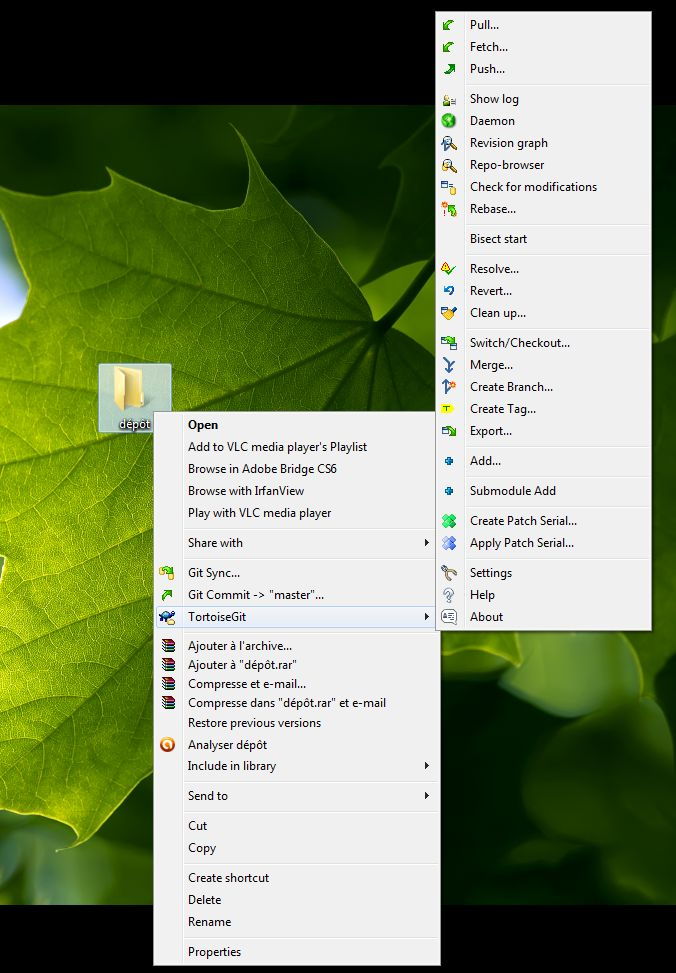
\includegraphics[scale=0.2]{../IMG/menuTG.jpg}
	\end{center}
	\caption{Tortoise Git : Le menu du depot}
	\label{Tortoise Git : Le menu du depot} 
\end{figure}
\newpage
\section{Un système de commits}

Git fonctionne un peu comme svn : par un système de version, ici appelés commit.\\
Pour commencer : créez un fichier nommé yoyo.txt et écrivez "Version 1" dedans.

A ce moment précis, vous considérez avoir bien travaillé et souhaitez \textbf{sauvegarder} votre travail dans git, de manière à le retrouver si jamais, plus tard, le fichier aurait un problème.

Nous allons donc créer une nouvelle version du projet.

\subsection{Indexer les fichiers}
Avant de créer un commit, nous devons dire à git quels fichiers doivent être pris en compte :
on appelle ça indexer les fichiers.
Indexer un fichier le mettra directement en cache, dans le dépôt.

\textbf{Attention : } Seuls les fichiers normaux et leur chemin sont mis en cache. Git en prend pas en compte les dossiers.\\
Si git veut nous créer un fichier sur notre ordinateur, si le dossier n'existe pas, il le fabrique.\\
Si on veut indexer un dossier vide, rien ne se passera.

\subsubsection{Par ligne de commande}
\begin{verbatim}
# Indexer le fichier1, le fichier2, et tous les fichiers du dossier3 (récursif)
$ git add <fichier1> [fichier2] [dossier3]

# Par exemple : indexe tous les fichier du dossier courant (et les ajoute au cache)
$ git add .

# Pour savoir quels sont les fichiers ajoutés, à ajouter, 
# modifiés (comparé au commit précédent)
$ git status
\end{verbatim}

Pour désindexer un fichier (supprimer le fichier et arrêter sa sauvegarde par le système de fichier), vous devrez passer par la commande git rm ou bien en supprimant au préalable le fichier et en utilisant l'option -A avec la commande git add.\\

Si vous souhaitez conserver le fichier dans votre système mais le retirer de l'index de git, il faut utiliser la commande git rm --cached

\subsubsection{Avec tortoise git}
Clic droit $\rightarrow$ Tortoise Git $\rightarrow$ Add

Tortoise git aide à l'indexation pendant le commit, il vous est en soi inutile de faire Add.\\
\newpage
\subsection{Créer un commit}
\subsubsection{Par ligne de commande}
\begin{verbatim}
# Créer un commit
$ git commit
\end{verbatim}

\textbf{Attention : } Vous allez entrer en mode texte (programme Vi) pour insérer un message.
Ici les lignes commançant par \# seront ignorées.
Pour éditer le texte, appuyez sur "i", pour arrêter l'édition, appuyez sur "Echap", pour valider le message :
arrêtez l'édition puis tapez ":wq"\\

Pour éviter de rentrer dans ce mode texte, vous pouvez écrire le message dans la commande :
\begin{verbatim}
# Créer un commit et tapez directement son message
$ git commit -m "Message"
\end{verbatim}

Pour indexer tous les fichiers qui ont été mis en cache :
\begin{verbatim}
# Créer un commit en indexant tous les fichiers mis en cache
$ git commit -a
\end{verbatim}

Vous pouvez aussi bien mélanger les options :
\begin{verbatim}
# Créer un commit en indexant tous les fichiers mis en cache
# et tapez directement son message
$ git commit -a -m "Message"
\end{verbatim}

\subsubsection{Par tortoise git}

Clic droit $\rightarrow$ Git Commit $\rightarrow$ "master"\\

Une fenêtre doit s'ouvrir contenant :
\begin{itemize}
\item Les fichiers mis en cache (avec une case cochée)
\item Les fichier non indexés (avec une case décochée)\\
\end{itemize}

La case indique s'il faut indexer ou non le fichier pour le commit à venir.
Si le fichier n'était pas en cache, il sera ajouté au dépôt et mis en cache\\

Une fois les fichiers choisis : tapez le message du commit (tentez d'être clair), signez, puis validez.\\

Vous pouvez aussi le faire directement depuis le log en faisant:
Clic droit $\rightarrow$ Tortoise git $\rightarrow$ Show log\\

Vous y verrez vos commits et les modifications courantes.\\
Pour créer un commit à partir de là : Clic droit sur "Working dir changes" $\rightarrow$ Commit
\newpage
\paragraph{Fenêtre de commit } Ici, le fichier toto.txt à été modifié, et le fichier nouveau.txt à été crée sans avoir encore été mis en cache/indexé.

\begin{figure}[h] 
	\begin{center}
		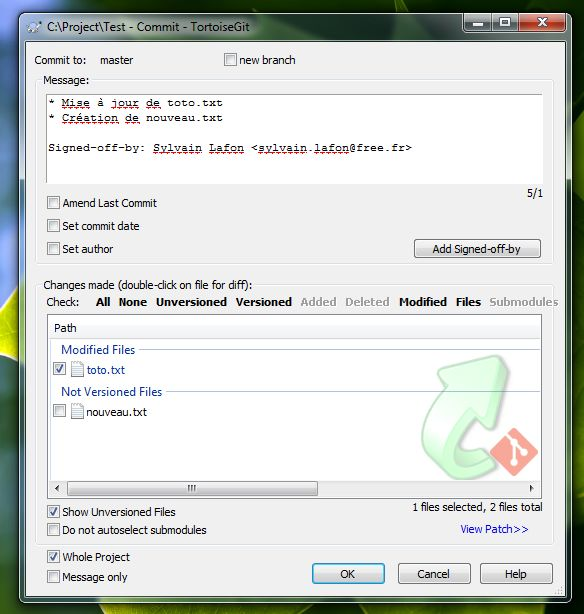
\includegraphics[scale=0.3]{../IMG/commit.jpg}
	\end{center}
	\caption{Tortoise Git : fenetre de commit}
	\label{Tortoise Git : fenetre de commit} 
\end{figure}

Pour ajouter le fichier nouveau, il suffit de cliquer sur la case à sa gauche.\\

\paragraph{Le log } Voici ce dont à quoi ressemble la fenêtre de log :

\begin{figure}[h] 
	\begin{center}
		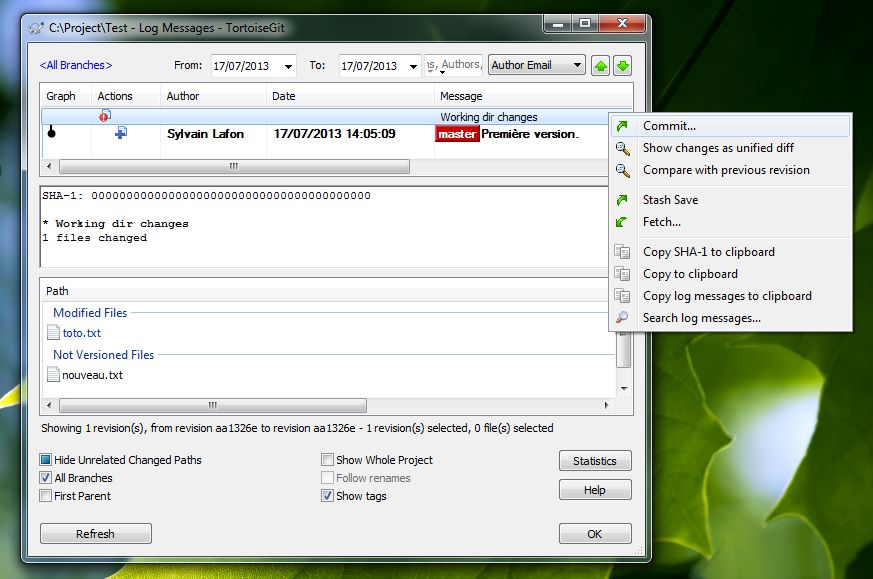
\includegraphics[scale=0.3]{../IMG/log.jpg}
	\end{center}
	\caption{Tortoise Git : fenetre de log}
	\label{Tortoise Git : fenetre de log} 
\end{figure}

Cette fenêtre doit être la fenêtre la plus importante de Tortoise git : elle permet d'afficher les commits en faisant leur graphe à leur gauche, en permettant, au clic droit de faire toutes les opérations que l'on verra.\\
Ici, un clic droit sur "Working dir. changes" permet de créer un commit,
on peut aussi faire des clics droit sur les branches, tags et commits.
\newpage
\subsection{Bien nommer les commits}

Idéalement, un commit devrait se présenter sous la forme suivante :
La première ligne devrait comporter moins de 50 caractères et résume les changements du commit.
Elle devrait être suivie d'une ligne blanche, puis des lignes qui décrivent plus en détail les différentes modifications.\\

Le texte situé au dessus de la ligne blanche est pris comme étant le titre du commit, utilisé dans git. (et Tortoise Git).\\
La commande git format-patch permet par exemple d'envoyer un commit par email et utilise le titre pour le sujet et le reste dans le corps du message.

\subsection{Se déplacer dans les commits}

Pour la suite du tutoriel,
faites deux nouveaux commits en modifiant le contenu de toto.txt

\subsubsection{Par ligne de commande}
\begin{verbatim}
$ git checkout <id>
\end{verbatim}

$<$id$>$ peut être un nom de branche, de tag ou bien l'id (SHA-1) du commit.
Pour connaitre les différents id de commit : 

\begin{verbatim}
$ git log --oneline --color --graph
\end{verbatim}

\subsubsection{Par tortoise git}
Clic droit $\rightarrow$ Tortoise git $\rightarrow$ Switch/Checkout
Une fenêtre apparait pour savoir vers où se déplacer, cochez "Commit" et ouvrez le log, cliquez sur la deuxième version puis "Ok", et "Ok".\\

Votre fichier a dû retrouver le contenu qu'il avait au deuxieme commit.\\

Vous pouvez aussi le faire directement depuis le log en faisant:
Clic droit $\rightarrow$ Tortoise git $\rightarrow$ Show log\\

Puis clic droit sur une version et "Switch/Checkout to this"
La version sur laquelle on se situe sera écrite en gras.
\newpage
\subsection{Référencer les commits importants : les tags}
Vous trouvez que certains commits sont très importants et vous y aimerez y accèder facilement, sans avoir à taper leur SHA-1 ? \\

Pour cela on utilise un tag. Il s'agit d'une simple référence à un commit, un nom.\\

Sur GitHub, une partie "Téléchargement" permet de télécharger le .zip du projet pour chaque tag !

\begin{figure}[h] 
	\begin{center}
		
\includegraphics[scale=0.4]{../IMG/tagsdl.jpg}
	\end{center}
	\caption{GitHub : les tags}
	\label{GitHub : les tags} 
\end{figure}

\subsubsection{Par ligne de commande}
Pour commencer, allez sur le commit en question, puis utilisez "git tag"
\begin{verbatim}
# On va sur le commit dont le SHA-1 débute par abcdef
$ git checkout abcdef

# On y crée un tag nommé : "v1.0"
$ git tag v1.0

# On peut désormais y accèder en tapant "v1.0"
$ git checkout v1.0

# Pour SUPPRIMER un tag :
$ git tag -d v1.0
\end{verbatim}

\subsubsection{Par Tortoise Git}
Et par le log et par le menu, on a "Create tag".\\

Pour supprimer un tag, on doit forcément aller dans le log de tortoise git, puis faire un clic-droit sur le tag (en jaune) avant de cliquer sur Supprimer.
\newpage
\section{Un système de branches}

Puisque nous pouvons travailler en parallèle où bien vouloir modifier un fichier à partir d'une version plus récente :
git utilise ce que l'on appelle des branches.\\

\subsection{Commits, branches et HEAD}

Par défaut, nous avons 3 choses :
\begin{verbatim}
A     B     C
* --- * --- *
        HEAD=master
\end{verbatim}

\begin{description}
\item[- Les commits : ] sont représentés par les * : A, B et C.\\
Ils ont chacun un identifiant SHA-1.\\
\item[- Les branches : ] ici, il n'y a que master.\\
Une branche fait parti de ce que l'on appelle une référence, dans git. Elles sont représentées par un fichier qui se situe dans .git/refs/heads et qui contient le SHA-1 du commit où elles se trouvent.\\
\item[- HEAD : ] Il s'agit de l'endroit sur lequel on est.\\
Unique, HEAD fait aussi parti de ce que l'on appelle une référence, mais celle-ci est particulière étant donné qu'elle peut à la fois pointer sur un commit, mais aussi sur une autre référence (ex: une branche).\\
Il est représenté par le fichier /.git/HEAD.\\
\end{description}

\textbf{Attention : }Si HEAD se trouve sur le même commit qu'une branche, cela ne veut pas dire que HEAD pointe forcément sur une branche !\\

Dans mes schémas, si HEAD ne pointe pas sur un commit mais sur une branche, j'utiliserai le symbole =. Dans le schéma ci-dessus : HEAD pointe sur master.
\newpage
Sur Tortoise Git, HEAD est représenté par le gras.
Si HEAD se trouve sur une branche, le nom de la branche en question est mis en rouge.\\

Lorsque l'on crée un commit, il est crée à partir du commit où se trouve HEAD, et il peut se passer deux choses :\\
\begin{itemize}
\item si HEAD pointe sur un commit : HEAD pointe sur le nouveau commit
\item si HEAD pointe sur une branche : la branche pointe sur le nouveau commit, HEAD pointe toujours sur la branche (la branche grandit)\\
\end{itemize}

\begin{verbatim}
A     B     C                A     B     C     D
* --- * --- *       ====>    * --- * --- *
    HEAD  master                   |   master
                                   ----------- *
                                              HEAD
          
A     B     C                A     B     C     D
* --- * --- *       ====>    * --- * --- * --- *
           HEAD                        master HEAD
          master                          
          
          
A     B     C                A     B     C     D
* --- * --- *       ====>    * --- * --- * --- *
        HEAD=master                        HEAD=master
        
\end{verbatim}

Dans le cas où l'on sort d'une branche non référencée, nous risquons de perdre tout les commits qu'elle apportait.
Pour éviter que cela n'arrive, nous allons commencer par apprendre à créer une nouvelle branche.

\begin{verbatim}
A     B     C     D            A     B     C     D
* --- * --- *                  * --- * --- *
      |   master       ====>         | HEAD=master
      ----------- *                  ----------- *
                 HEAD                         (perdu)
\end{verbatim}
\newpage
\subsection{Créer une branche}
\subsubsection{Par ligne de commande}

Par défaut, la branche que vous créerez se situera à l'endroit où se trouve HEAD.
Il y a deux méthodes pour créer une branche :

\begin{verbatim}
# Créer une branche et y faire pointer HEAD
$ git checkout -b <nom_branche>

# Créer une branche sans y faire pointer HEAD
$ git branch <nom_branche>
\end{verbatim}

\subsubsection{Par Tortoise Git}
\begin{itemize}
\item Clic droit $\rightarrow$ Tortoise Git $\rightarrow$ Create branch
\item Log $\rightarrow$ Clic droit sur une version $\rightarrow$ Create branch at this version
\item Lors d'un commit : case "New branch", la branche sera crée et HEAD pointera dessus avant que le commit ne se crée
\end{itemize}

\subsubsection{Résultat}
\begin{verbatim}
A     B     C                A     B     C     D
* --- * --- *       ====>    * --- * --- *
    HEAD  master                   |   master
                                   ----------- *
                                              HEAD                                              

                    ====>    A     B     C     D
                             * --- * --- *
                                   |   master
                                   ----------- *
                                         HEAD=maBranche
\end{verbatim}

\newpage
\subsection{Déplacer HEAD}

Il y a plusieurs méthodes pour faire déplacer HEAD :\\

\begin{verbatim}
# Déplace HEAD proprement, mélange les modifications en cours avec  
# celles induites par le déplacement dans les versions.
# Empêche le déplacement en cas de conflits dans le mélange des modifications.
$ git checkout <ref>

# Déplace HEAD en SUPPRIMANT toutes les modifications en cours.
$ git reset --hard <ref>

# Déplace HEAD mais conserve les fichiers du précédent commit et les indexe
# Les modifications en cours seront la différence entre le commit cible 
# et le commit précédent en plus des modifications qu'il y avait
$ git reset --mixed <ref>

# Déplace HEAD mais conserve les fichiers du précédent commit et ne les indexe pas
# Cela revient à modifier /.git/HEAD
$ git reset --soft <ref>
\end{verbatim}

Il est possible de faire l'ensemble de ces opérations avec tortoise git à partir du log : Faites un clic droit sur la branche ou le commit qui vous intéresse et choisissez Checkout ou Reset. Si vous choisissez reset, vous aurez le choix entre les trois modes.

\newpage

\subsection{Fusionner la branche courante}

Bien évidemment, si on ne pouvait pas stocker les changements quelle apporte dans la branche principale, la création d'une nouvelle branche ne servirait à rien.
Nous allons donc apprendre à mettre à jour une branche en la fusionnant avec HEAD.

Pour pouvoir fusionner deux branches il faut, pour commencer, que la branche à fusionner apporte des changements à la branche courante.\\

Par exemple :
\begin{verbatim}
A       B       C
* ----- * ----- *
      aMerger 
            HEAD=master
\end{verbatim}

Il est absolument inutile dans ce cas de fusionner aMerger dans master !
master contient déjà toutes les modifications de aMerger.
\newpage
\begin{verbatim}
A       B       C               A       B       C
* ----- * ----- *               * ----- * ----- *
   HEAD=master          ====>               HEAD=master
              aMerger                         aMerger
\end{verbatim}

Là, par contre, bien que master n'apporterait rien à aMerger, ici,
aMerger contient des modifications que master n'a pas. Fusionner master et aMerger permettrait de mettre à jour master.

\begin{verbatim}
A     B     C     D             A        B        C        D         M
* --- * --- *     *             * ------ * ------ * ---------------- *      
      | HEAD=master     ====>            |                           |
      ----------- *                      ----------------- * ---------
                aMerger                                 aMerger  HEAD=master
                                                      (fusionnée)
\end{verbatim}

Ici, les deux branches ont eu des changements parallèles : une véritable fusion entre les fichiers à lieu, ce qui crée un commit de fusion.
Git est assez puissant et arrive facilement à faire la part des choses, cependant parfois les mêmes endroits des mêmes fichiers sont modifiés, on appelle ça un conflit : il faut, dans ce cas, le résoudre à la main. On en parlera plus tard. \\

Donc maintenant, comment fusionner les branches ?
\subsubsection{En lignes de commande}
\begin{verbatim}
# Faites attention que vous n'ayez rien à commiter !
$ git status

# D'abord on se place sur la branche que l'on veut
$ git checkout aMettreAJour

# Puis on fusionne !
$ git merge aMerger

# Résultat
$ git log --oneline --color --graph
\end{verbatim}

\subsubsection{Par Tortoise git}
Vous devriez être déjà plus familier avec l'interface.
Le bouton à appuyer s'appelle "Merge".
Il faut tout d'abord veiller à bien être sur la branche qui recevra la fusion.
On peut trouver le bouton et dans le log et dans le menu clic-droit.
\newpage
\subsection{Résoudre les conflits}

Arg, votre fusion ne s'est pas faite toute seule et git vous supplie de l'aider ?
Pas de soucis, on va les résoudre ces conflits !!

Lorsque git ne sait pas quoi faire, il va écrire localement tous les confits dans le fichier

Par exemple :
Ecrivons dans notre fichier toto :
\begin{verbatim}
A
B
C
D
E
\end{verbatim}

Créons un commit, et retournons au commit précédent\\

\textbf{Astuce} Pour la ligne de commande : HEAD$^{\bigwedge}$1 indique : "un commit avant HEAD"\\

Créons une nouvelle branche "troll" écrivons dans le fichier toto :
\begin{verbatim}
A
bbbbb
C
ddddd
E
\end{verbatim}

Créons un commit, nous devrions avoir un graph qui ressemble à ça :

\begin{verbatim}
                     A      B      C
anciens commits ---- * ---- *
                     |    master
                     ------------- *
                               HEAD=troll
\end{verbatim}

Maintenant, retournons (HEAD) sur master et fusionnons troll à HEAD(=master).

La fusion se place pas comme prévue (enfin..) et git vous indique qu'il a besoin d'aide.
A ce moment précis, toutes les modifications apportées par troll sont indexées, et les fichiers non fusionnés sont notés comme "conflictueux"
\newpage
Git, pour vous aider, à écrit dans toto de cette manière :
\begin{verbatim}
A
<<<<<<< HEAD
B
C                                <-- Partie telle qu'elle est dans HEAD
D
=======
bbbbb
C                                <-- Partie telle qu'elle est dans troll
ddddd
>>>>>>> troll
E
\end{verbatim}

Pour résoudre le conflit vous devez alors supprimer les annotations supplémentaires et fusionner la partie problématique.
Pour indiquer à git que le conflit est résolu il suffit d'indexer le fichier (git add) ou de le supprimer (git rm) et pour finir la fusion, il faut créer le commit de fusion (il est impossible de faire de commit s'il reste des fichiers conflictueux)

\subsubsection{En ligne de commande}

Vous pouvez faire revenir un fichier selon l'une ou l'autre branche à l'aide de checkout :
\begin{verbatim}
# Marque toto.txt comme résolu :
$ git add toto.txt

# Résout le conflit en prenant le fichier de HEAD(=master)
$ git checkout --ours toto.txt

# Résout le conflit en prenant le fichier de la branche à fusionner (troll)
$ git checkout --theirs toto.txt
\end{verbatim}

\subsubsection{Sous tortoise git}

Tout comme en ligne de commande, sous Tortoise Git, il y a des outils facilitant la résolution des conflits. Des outils de feignants certes, mais bien utiles.\\
Après la tentative de fusion, git vous propose de "Résoudre" les conflits, si vous acceptez : la fenêtre de commit normale apparait (sinon il suffit de cliquer sur "Commit")\\

Ici, Tortoise git propose trois choses (clic droit sur les fichier à conflit) :
\begin{itemize}
\item Résoudre le conflit (il faut faire les modifications à la main avant)
\item Résoudre le conflit en prenant la version locale (celle de HEAD)
\item Résoudre le conflit en prenant la version distante (celle de troll)\\
\end{itemize}

Bien sûr il reste aussi possible de le supprimer.
\newpage
\subsection{Supprimer une branche}

Pour commencer : on ne peut pas supprimer une branche si HEAD est dessus, ensuite, pour supprimer une branche \textbf{sans forcer}, elle doit être fusionnée, par exemple :
\begin{verbatim}
__________________________________________________

 A        B        C        D         M
 * ------ * ------ * ---------------- *      
          |                           |            
          ----------------- * ---------
                         aMerger  HEAD=master
                       (fusionnée)
                       
> Aucun risque de supprimer aMerger
__________________________________________________
                       
 A        B        C        D        
 * ------ * ------ *      
          |    HEAD=master                         
          |                                        
          ----------------- *                      
                         branche1 (fusionnée à branche2)
                         branche2 (fusionnée à branche1)

> Aucun risque de supprimer branche1 ou branche2
__________________________________________________

 A        B        C        D        
 * ------ * ------ *      
          |    HEAD=master                         
          |                                        
          ----------------- *                      
                         branche1

> Supprimer branche1 risque de perdre D .       
\end{verbatim}
(Un commit perdu n'est pas tout de suite supprimé : il restera accessible avec son SHA-1 quelques temps. (cf : git prune))\\

Si la branche n'est pas fusionnée, il va falloir forcer, à ce moment là, on peut supprimer la branche "aMerger" sans aucun problème, et sans perdre quoi que ce soit.
\newpage
\subsubsection{En ligne de commande}
\begin{verbatim}
# On s'assure de ne pas être sur aMerger
$ git checkout master

# On la supprime (si fusionnée)
$ git branch -d aMerger

# On la supprime (en forcant)
$ git branch -D aMerger
\end{verbatim}

Par sécurité, il est conseillé de ne jamais forcer (sauf si vous vous fichez de perdre le travail qui n'a pas été fusionné).

\subsubsection{Avec tortoise git}
Sur la version de Tortoise git que j'ai actuellement : on est obligé d'ouvrir le log pour supprimer une branche (clique-droit sur une branche (en vert))\\

\textbf{Attention} : Cela forcera la suppression automatiquement, alors soyez vigilants !

\newpage
\section{Un dépôt en ligne}
L'un des grands avantages d'utiliser git, en plus de pouvoir gérer facilement les versions hors-ligne (ce qui le démarque de \acl{svn}), c'est aussi la possibilité de synchroniser ses branches sur un serveur en ligne rendant ainsi possible la mise en commun des différentes versions\\

Lorsque l'on lie notre dépôt à un dépôt distant, on peut :
\begin{description}
\item[- fetch :]Recevoir les branches en ligne (et les commits de différence)
\item[- push :] Créer/Fusionner (commit de fusion interdit) une de nos branches, dans le serveur
\end{description}

Commençons par lier notre dépôt à un dépôt en ligne.

\subsection{Lier un dépôt local à un dépôt serveur}
\subsubsection{Par ligne de commande}
\begin{verbatim}
$ git remote add <nom identifiant du dépôt> <adresse du dépôt>

# Par défaut on appelle le premier identifiant "origin"

# Exemple pour github, par ssh :
$ git remote add origin git@github.com:nomUtilisateur/nomDepot.git

# Exemple pour github, par https :
$ git remote add origin https://github.com/nomUtilisateur/nomDepot.git
\end{verbatim}

\subsubsection{Par Tortoise git}
Clic droit $\rightarrow$ Tortoise git $\rightarrow$ Settings $\rightarrow$ Git $\rightarrow$ Remote\\

Ici, on renseigne les champs "Remote" et "URL", avant d'appuyer "Add New/Save" puis "Ok"\\

Par exemple : "origin" et "git@github.com:nomUtilisateur/nomDepot.git" pour github

\newpage
\subsection{Créer un clone d'un dépôt en ligne}

Créer un clone d'un dépôt permet d'obtenir un dépôt local identique au dépôt en ligne, directement lié avec le dépôt en ligne. (l'identifiant sera "origin").

\subsubsection{Par ligne de commande}
\begin{verbatim}
$ git clone <adresse du dépot> [nom du dossier (optionnel)]

# Exemple pour github, par ssh :
$ git clone git@github.com:nomUtilisateur/nomDepot.git

# un dossier "nomDepot" sera crée

# Exemple pour github, par ssh :
$ git clone git@github.com:nomUtilisateur/nomDepot.git nomDossier

# un dossier "nomDossier" sera crée
\end{verbatim}

\subsubsection{Tortoise git}
Clic droit en dehors d'un quelconque dépôt, puis Clone.
On remplit l'url, et c'est parti !

\subsection{Récupèrer les différences avec le serveur}
Pour récupèrer les modifications qui se sont faites en ligne, il suffit de faire un "fetch"
(git fetch).

Si des commits existent en ligne mais pas en local, ils seront téléchargés.

Exemple :
\begin{verbatim}

          A     B     C
local :   * --- * --- *     
                  HEAD=master

ORIGIN    A     B     C     D
remote :  * --- * --- * --- *
                        HEAD=master
   
<<FETCH ORIGIN>>

          A        B        C        D         
local :   * ------ * ------ * ------ *
                        HEAD=master
                          origin/HEAD=origin/master
\end{verbatim}

Pour mettre à jour master, il suffit de faire un merge de origin/master !\\

Faire les deux opérations à la suite, c'est faire faire un pull (git pull)

\subsection{Fusionner une branche distante}
Pour mettre à jour le serveur, faire un Push, il faut au préalable que notre branche soit déjà fusionnée avec la branche à fusionner.. concrètement :
\begin{verbatim}
A     B     C
* --- * --- *             <-- Déjà à jour.
          master
       origin/master

A     B     C
* --- * --- *             <-- Possible
          master   
  origin/master
  
A     B     C
* --- * --- *             <-- Pas possible (inutile)
          origin/master   
    master
           
A     B     C     D
* --- * --- *             <-- Pas Possible (non fusionnée : conflit possible)
      |   master  
      ----------- *     
            origin/master
\end{verbatim}

\subsection{Astuce : Le protocole habituel}
Habituellement, lorsque l'on veut envoyer notre version en ligne, on fait, ces opérations dans l'ordre :

\begin{enumerate}
\item ADD : On indexe les modifications et on met en cache les nouveaux fichiers
\item COMMIT : On crée un commit, une version
\item FETCH : On récupère la version en ligne
\item MERGE : On fusionne la version en ligne avec la version locale
\item PUSH : On envoie la nouvelle version locale en ligne\\
\end{enumerate}

Puisque un commit peut faire un "add" et que le fetch et merge se font avec la commande "pull", on peut résumer le protocole à :\\

\begin{enumerate}
\item COMMIT EN INDEXANT (commit -a / les cases de tortoise)
\item PULL (FETCH + MERGE)
\item PUSH
\end{enumerate}
\newpage
\subsection*{Lignes de commande}
\begin{verbatim}
# récupèrer pour toutes les remotes
$ git fetch 

# récupèrer que pour origin
$ git fetch origin

# récupèrer pour toutes les remotes et merger toutes les branches
$ git pull

# récupèrer que pour origin et merger toutes les branches
$ git pull origin

# récupèrer que pour origin et ne merger que master
$ git pull origin master

# tout envoyer sur toutes les remotes
$ git push

# tout envoyer sur origin
$ git push origin

# envoyer master sur origin
$ git push origin master

# envoyer master en tant que "maBranche" sur origin
$ git push origin master:maBranche
\end{verbatim}

\subsection{Supprimer une branche distante}
\subsubsection{Par ligne de commande}
On va utiliser l'option --delete de push :
\begin{verbatim}
# détruit et la branche locale origin/maBranche et la branche maBranche d'origin
$ git push origin --delete maBranche
\end{verbatim}
\subsubsection{Par tortoise git}
Dans le log, clic droit sur une remote/branche et supprimer : une popup apparaîtra pour savoir s'il faut ou non supprimer ET la branche locale (remote/branche) ET la branche "branche" sur le dépôt en ligne.

% Fait sauter une page dans le Table of contents
\addtocontents{toc}{\protect\newpage}
	\part{Installation et configuration d'un serveur git}
\chapter{Créer le serveur}

Fini Github ! A Manzalab, nos projets sont confidentiels et il existe des moyens gratuits d'avoir un serveur git privé, si nous avons un ordinateur prêt à endosser le rôle de serveur (cela implique, qu'une fois éteint ou la connexion coupée, le dépôt "en ligne" sera inaccessible).\\

Créer un dépôt serveur git est vraiment tout simple, cependant, la connexion à ce dépôt est un peu plus problèmatique..\\
Alors pour simplifier les choses, nous allons utiliser une interface simplifiée : Gitstack.

\section{Pour windows : GitStack}
Gitstack est une interface gérant l'accès aux dépôts via http.\\
Elle crée les dépôts, et permet à des utilisateurs et groupes à s'y connecter.\\

\subsection{Installer Gitstack}

Commençons par l'installer (sur la machine serveur) en allant sur son \href{http://gitstack.com/}{Site officiel}\\

Durant l'installation, on vous demandera d'installer git. Il est fortement recommandé de l'installer.\\

Une fois installé et lancé, prenez votre navigateur favori et allez à l'adresse : \href{http://localhost/gitstack/}{http://localhost/gitstack/}\\
Vous y apercevrez le panneau d'administration de Gitstack, ce dont on parlera durant tout le chapitre.
\newpage
\subsubsection{Allez-y ! C'est permis !}
Vous serez en mode trial : une sorte de mode dans lequel vous pourrez tout faire.\\
La license de GitStack stipule que même la version payante.. est gratuite, et que l'on peut modifier les fichiers chez nous.
Ainsi, lorsque votre mode trial sera passé, vous pourrez le réinitialisant en supprimant et en recréeant le fichier core se situant dans le dossier /data (GitStack regarde la date de création du fichier.. ..qui ne contient rien)\\

Une petite copie appuyant mes propos :
\begin{verbatim}
GitStack
Copyright (C) 2012 Smart Mobile Software

This program is free software: you can redistribute it and/or modify
it under the terms of the GNU General Public License as published by
the Free Software Foundation, either version 3 of the License, or
(at your option) any later version.

This program is distributed in the hope that it will be useful,
but WITHOUT ANY WARRANTY; without even the implied warranty of
MERCHANTABILITY or FITNESS FOR A PARTICULAR PURPOSE. See the
GNU General Public License for more details.

You should have received a copy of the GNU General Public License
along with this program. If not, see <http://www.gnu.org/licenses/>.
\end{verbatim}

Vous pouvez donc modifier tout fichier en toute légalité, selon l'auteur.

\newpage
\subsection{Administrer Gitstack}

Gitstack contient en somme deux choses :
\begin{itemize}
\item Les dépôts
\item Les utilisateurs\\
\end{itemize}

Gitstack nous permet dans son interface, de :
\begin{itemize}
\item créer et supprimer des dépôts
\item modifier les privilèges des groupes et utilisateurs pour un dépôt donné
\item créer/supprimer des utilisateurs (couple login/mot de passe) 
\item créer/supprimer des groupes (ensemble d'utilisateurs)
\end{itemize}

\section{Autres moyens}

Bien sûr, nous n'avons vu là qu'une méthode, et qui ne fonctionne que sous windows, mais nous pouvons également utiliser un serveur ssh (OpenSSH, par exemple), ou notre propre serveur http.\\

Avec OpenSSH, il vous faudra recueillir les clés publiques RSA de vos utilisateurs et les stocker dans les différents fichiers authorizedkeys.\\
De nombreux tutoriels existent sur internet, je vous laisse les trouver.

\chapter{Un dépôt serveur}
\section{Créer un dépôt serveur}
Pour créer un dépôt serveur, nous avons utilisé Gitstack, mais nous pouvons aussi en créer un avec tortoise git ou en ligne de commande.\\

\textbf{Avec tortoise git}, il suffit de faire un clic-droit sur un dossier vide (par convention les noms de ces dossiers se terminent par ".git") et faites "Make it bare". si votre dossier se fini par .git, la case est déjà cochée par défaut.\\

\textbf{En ligne de commande}, allez dans le nouveau dépôt puis tapez :
\begin{verbatim}
$ git init --bare
\end{verbatim} 

\section{Administrer le dépôt}
Contrairement au dépôt local, le dépôt serveur n'est en fait qu'un .git !\\
Celui-ci contient presque exactement toutes les mêmes informations que nos dépôts locaux :
\begin{itemize}
\item Le fichier config permet de gérer les options de git pour le dépôt
\item Le fichier description décrit le dépôt
\item Les autres fichiers sont aussi présents en local, par exemple on retrouve le HEAD du serveur (utile si on s'aperçoit d'une erreur en ligne)
\end{itemize}
	\part{Utilisation avancée de git}

\chapter{Notions avancées}
\section{Empêcher l'indexation avec .gitignore}

.gitignore est un fichier permettant d'empêcher l'indexation de fichiers (git add).\\
Ils fonctionnent sur le principe suivant : Chaque ligne du fichier contient une expression régulière. Si un fichier à un chemin qui correspond à l'une des expressions régulières d'un .gitignore (chemins relatifs), alors le fichier ne sera pas indexé (s'il ne l'est pas déjà).

Pour retirer un fichier du cache, il suffit d'utiliser git rm :
\begin{verbatim}
# Supprime DU CACHE tous les fichiers du dossier.
$ git rm -rf --cached .

# Ajoute dans le cache tous les fichiers du dossier.
$ git add .

# Les deux commandes mises côte à côte permet de sortir
# du cache tout ce qui est dans le .gitignore.
\end{verbatim}

Sous Tortoise git :\\

Clic-droit sur un fichier $\rightarrow$ Tortoise Git $\rightarrow$ Delete (keep local)

\section[Optimisez votre dépôt avec le Garbage Collector]{Optimisez votre dépôt avec le GC}

git gc et git prune

\section{Comparer deux versions}

git diff et git log
\newpage
\section{Retournons vers le futur}
\subsection{Reprendre la version d'un ou plusieurs fichiers précis}

Car oui, il est possible \textbf{sans tricher\footnote{Tricher : Se prendre la tête en se déplaçant dans les commits et des copiés collés}} de faire revenir juste un fichier en arrière, et ce, grâce à checkout !

\begin{verbatim}
# Remet fichier tel qu'il est dans <id> (ex : master, SHA-1, HEAD, tag)
$ git checkout <id> /chemin/fichier

# Remet fichier tel qu'il est dans le commit dans lequel HEAD est.
$ git checkout -- /chemin/fichier
\end{verbatim}

-- permet de séparer les $<$id$>$ des fichiers. Dans le cas où une branche s'appelle fichier.txt (oui, je sais), cela permet de retirer l'ambiguïté\\

Avec Tortoise git, on appelle ça : faire un Revert.

\begin{itemize}
\item Clic-droit sur un fichier de Working dir changes : annule les modifications courantes d'un fichier
\item Clic-droit sur un fichier d'un commit : fait revenir un fichier tel qu'il était dans le commit en question.
\end{itemize}

\subsection{Annuler un ou plusieurs commits}
Une autre commande peut-être utilisée si l'on veut prendre tous les fichiers à la fois : revert. Tortoise Git permet de le faire en faisant un clic doit sur le(s) commit(s) en question.

\begin{verbatim}
# Annule les changements du commit <id> et crée un commit.
$ git revert <id>

# Annule les changements du commit <id> sans créer de commit
# il faudra le faire nous même.
$ git revert -n <id>
$ git commit -m "Revert"
\end{verbatim}

\paragraph{Attention : } Revert ne fonctionne qu'avec des commits et se termine en créeant un commit !

\newpage
\subsection{Annuler les modifications en cours}

Il y a plusieurs méthodes pour faire ça : checkout et reset :
(l'option hard permet d'appliquer l'annulation sur les fichiers en plus de HEAD)

\begin{verbatim}
$ git reset --hard HEAD
$ git checkout -- .
\end{verbatim}

\subsubsection{Annuler un commit non partagé}
Utilisé sur un commit (et non sur HEAD), cela permet de supprimer le commit de l'arbre.
Si le commit a été déjà partagé, cela ne servira à rien et risque de poser des problèmes, dans ce cas il faudra utiliser revert (mais il apparaîtra toujours dans l'arbre).\\

Vous connaissez maintenant les différences de comportement entre checkout, revert et reset.



\newpage
\section{Sélectionner un commit à partir d'un autre}
\subsection{Identifier un commit précis}

Comme je vous l'avais dit, il y a plusieurs moyens de se déplacer : \\

Par exemple :\\
\begin{itemize}
\item En écrivant le SHA-1 d'un commit
\item En écrivant le nom d'une branche
\item En écrivant le nom d'un tag\\
\end{itemize}

Mais ce n'est pas tout !\\

On peut aussi :
\begin{itemize}
\item Se déplacer dans un commit à partir d'un autre commit
\item Se déplacer dans un commit en fonction de l'historique (n-ième opération, ou temps)
\end{itemize}

\subsubsection{Se déplacer à partir d'un commit}

Nous avons là deux symboles : \textasciicircum et \textasciitilde\\
HEAD\textasciicircum1 et HEAD\textasciitilde1 signifient la même chose : le commit précédent.\\

Avec un chiffre supérieur à 1, la différence se voit :
\begin{itemize}
\item HEAD\textasciicircum2 signifie : aller au second parent de HEAD (commit de merge)
\item HEAD\textasciitilde2 signifie : aller au (premier) parent du (premier) parent de HEAD\\
\end{itemize}

Ainsi, master\textasciitilde2 et master\textasciicircum\textasciicircum sont équivalents.\\
On peut aussi bien écrire : master\textasciicircum\textasciicircum\textasciitilde3\textasciicircum2 (ce qui revient à master\textasciitilde5\textasciicircum2, pour le coup)\\

\paragraph{Remarque :} Ecrire master\textasciicircum3 serait voué à l'echec.

\newpage
\subsubsection{Se déplacer à partir de l'historique}

Afin de connaître l'historique des références d'une branche ou de HEAD, on peut utiliser : git reflog.\\

Exemple : 
\begin{verbatim}
$ git reflog
734713b... HEAD@{0}: commit: fixed refs handling, added gc auto, updated
d921970... HEAD@{1}: merge phedders/rdocs: Merge made by recursive.
1c002dd... HEAD@{2}: commit: added some blame and merge stuff
1c36188... HEAD@{3}: rebase -i (squash): updating HEAD
95df984... HEAD@{4}: commit: # This is a combination of two commits.
1c36188... HEAD@{5}: rebase -i (squash): updating HEAD
7e05da5... HEAD@{6}: rebase -i (pick): updating HEAD

# git show montre le commit pointé
$ git show HEAD@{3}

# Si vous tapez trop loin, ça ne marchera pas.
\end{verbatim}

Comme vous pouvez le voir : on peut utiliser le symbole @ pour connaître le commit (le sha1 à côté) que pointait la référence au moment donné.

En plus d'utiliser un chiffre pour récupèrer la n-ième opération, on peut aussi bien utiliser une date :

\begin{verbatim}
$ git show HEAD@{yesterday}
$ git show HEAD@{2.months.ago}
$ git show master@{1 month 2 weeks 3 days 1 hour 1 second ago}
$ git show mybirth@{1992-09-29 23:00:00}

# Si vous tapez trop loin, ça ne marchera pas.
\end{verbatim}

\newpage
\subsection{Identifier un ensemble de commits}
\subsubsection*{Les deux points : ..}
Les deux points représentent la portée entre deux commits, par exemple :
branche1..branche2 représente tous les commits qui sont référencés dans branche2 mais pas dans branche1

Exemple :
\begin{verbatim}
A     B     C     D     E     F     G
* --- * --- * --- * --------- *
            |               master
            ----------- * --------- *
                                   test
                                   
$ git log master..test
G
E

$ git log test..master
F
D
\end{verbatim}

\subsubsection*{--not et \textasciicircum}
Certes le symbole .. est utile, mais parfois, on a besoin d'utiliser plus de deux branches.\\
Pour cela on peut utiliser le --not (ou \textasciicircum).

Exemple :
\begin{verbatim}
# Equivalents :
$ git log master..test
$ git log ^master test
$ git log test --not master

# Equivalents :
$ git log master test --not origin/master
$ git log master test ^origin/master

\end{verbatim}

\newpage
\subsubsection*{Les trois points : ...}

Les trois points représentent tous les commits entre deux références sauf ceux qui sont accessible à partir des deux références.\\

Exemple :
\begin{verbatim}
A     B     C     D     E     F     G
* --- * --- * --- * --------- *
            |               master
            ----------- * --------- *
                                   test
                                   
$ git log master...test
D
E
F
G

$ git log test...master
D
E
F
G

$ git log --left-right test...master
> D
< E
> F
< G
\end{verbatim}

\subsubsection{La portée chez Tortoise Git}

En maintenant Ctrl appuyé, dans le log, il est possible de selectionner plusieurs commits.\\
Dans le cas où on en selectionne deux, tortoise git nous propose un sous-log des commits en fonction de .. ou de ... !
\newpage
\section{Sauvegarder temporairement avec stash}

stash permet de sauvegarder l'état de l'index et des fichiers dans une pile (une liste de "stashes". Lorsque l'on y met un stash, il rentre en première position, lorsque l'on sort un stash, on retire celui en première position et on va avancer les autres) \\

Il y a plusieurs commandes principales (accessibles avec Tortoise Git) :
\begin{description}
\item[- Stash show/list : ]montre l'état de la pile
\item[- Stash save : ]sauve l'état courant des dossiers et de l'index et pousser ces objets dans la pile.\\
L'état des dossiers et de l'index sera remis tel qu'il était dans le commit
\item[- Stash pop : ]fusionne l'état courant des dossiers et de l'index avec celui sauvé et enleve ces objets de la pile.
\item[- Stash apply : ]fusionne comme avec pop mais ne retire rien de la pile
\item[- Stash drop : ]retire de la pile sans fusionner (perd les changements)
\item[- Stash clear : ]drop tout.\\ 
\end{description}

Afin de mieux comprendre comment utiliser ces commandes, nous allons prendre un petit exemple.

\newpage
\subsection{Application : le quickfix}
Imaginons que nous ayons un commit "SUR", que nous sommes en train de travailler sur le projet, et que le travail en cours est rempli de problèmes.\\
Tout-à-coup quelqu'un nous demande de fixer un problème du commit "SUR". Comment faire ?
\subsubsection{Vieille école : la création d'une branche temporaire}
Vous ne connaissiez pas stash et vous décidez donc de sauver votre travail en cours dans une nouvelle branche "unstable".\\
Vous allez donc y faire votre commit "en cours" (oui, du coup, c'est pas un BON commit) et allez retourner sur le commit "SUR", y faire votre fix, puis commiter le changement pour finalement retourner travailler sur votre branche, après y avoir fusionner le fix.\\

En somme, vous auriez fait ça :\\
\begin{verbatim} 
 SUR   ENCOURS   FIX    MERGE
- * ----- * ------------- * -
  |    (pwerk)            |
  --------------- * -------
               master  unstable
               
Plus tard :

 SUR   ENCOURS   FIX    MERGE  FEATURE
- * ----- * ------------- * ----- * -
  |                       |     master
  --------------- * -------
                 
\end{verbatim}

Résultat : vous avez deux commits buggés, où du travail est en cours de rédaction et dans lequel l'application pourrait poser problème. Ensuite, le travail effectif de FEATURE se situe sur trois commits distincts : entre SUR et ENCOURS, entre ENCOURS et MERGE (normalement, rien n'y est fait là) et enfin entre MERGE et FEATURE.\\

Autrement dit, si on souhaite localiser un problème cela promet d'être compliqué, et on risque de prendre nos deux commits pour des versions sures..
\newpage
\subsubsection{Nouvelle méthode : stash}

Avec stash, vous commencez par sauver vos changements en faisant stash save.\\
Vos changements sont retirés et vous êtes directement sous SUR, vous allez donc directement corriger votre problème. Une fois le fix terminé, vous le commitez puis pour continuer à travailler, vous allez faire un stash pop : Votre fix se fusionnera avec votre précédent stash, et vous pourrez terminer tranquillement votre travail.\\

Du côté de notre arbre, cela donne :
\begin{verbatim}
 SUR     FIX
- * ----- * -
        master
        
Plus tard :

 SUR     FIX   FEATURE
- * ----- * ----- * -      
                master
      
\end{verbatim}   

Dans cet arbre, les trois commits sont bons, on peut partir de SUR, FIX et FEATURE sans soucis. Les changements liées à la feature sont dans le commit FEATURE, le fix est bien dans FIX et rien n'est séparé.\\

Schématiquement, cela revient presque au même, en plus simple rapide et efficace :       
\begin{verbatim}
SUR --> TRAVAIL --> SUR --> FIX --> TRAVAIL+FIX --> FEATURE 
                 |               |
                 ---- TRAVAIL ----
                 
   edits       stash   edits    stash          edits
               (save) (commit)  (pop)         (commit)
\end{verbatim}

\subsection{Conflit lors du stash pop}

En cas de conflit, le pop est considéré raté et si l'outil de fusion a fait son travail,
le stash est toujours dans la pile. Une fois le conflit résolu vous devrez donc faire un stash drop (le retirer à la main)\\

\textbf{Attention : } Si vous refaites un stash pop, git tentera de fusionner la version fraîchement fusionnée avec l'ancien travail sauvé, ce qui fabriquera, dans ce cas, forcément un conflit, qui plus est : inutile !
%\section{Travailler sur un dépôt en lecture seule}
\subsection{Cloner un dépôt serveur}

git fork

\subsection{Soumettre votre travail pour le dépôt original}

 % Exclusif github ?
\newpage
\section{Ajoutez un dépôt.. ..dans votre dépôt}

%Pour faire cela, nous avons deux méthodes :
%\begin{description}
%\item[- git submodule : ] Va créer un nouveau dépôt git, dans un dossier donné, mais stocke sont propre .git dans le .git du dépôt parent (dans .git/modules). Les différents sous-dépôts seront référencés dans un fichier .gitmodules situé à la racine du dépôt parent. Pour manipuler ce sous dépôt il suffit de s'y rendre et d'utiliser les commandes git (/Tortoise Git) habituelles\\
%\item[- git subtree : ] Méthode la plus élégante et rétro-compatible, mais pas vraiment user-friendly. Pour manipuler tout ça, il faudra passer par de nouvelles commandes.. ..qui ne sont pas intégrées à Tortoise Git. C'est pour cela que je n'en parlerai pas dans ce tutoriel.\\
%\end{description}
%
%Pour en savoir plus sur git subtree et les différences entre ces méthodes, je vous conseille d'aller ici :
%\begin{itemize}
%\item Le man de git-subtree
%\item Alternatives To Git Submodule: Git Subtree 
%\end{itemize}

Pour cela nous allons créer un sous-dépôt, un 'submodule'.\\
Un sous-dépôt est un dépôt dont le .git se trouve dans le .git du parent dans le dossier modules, pour être précis.\\
La racine du sous-dépôt doit être l'un des dossiers du dépôt parent. Les différents sous-dépôts étant référencés dans un fichier .gitmodules se situant à la racine du dossier parent.\\

Voici un schéma de l'arborescence que l'on peut avoir :\\

\dirtree{%
 .1 /.
 .2 CheminVers/.
 .3 MonProjetGit/\\.
 .4 UnDossier1/.
 .4 UnFichier2.
 .4 UnAutreFichier3\\.
 .4 UnAutreDossier4/.
 .5 UnFichier5.
 .5 MonSousDepotGit/.
 .6 .git.
 .6 UnFichier6\\.
 .4 .gitmodules\\.
 .4 .git/.
 .5 modules.
 .6 UnAutreDossier4/.
 .7 MonSousDepotGit/.
 .8 (équivalent du .git du sous dépot)\\.
 .5 (d'autres choses)\\.
}

Ici, Le dossier /CheminVers/MonProjetGit/UnAutreDossier4/MonSousDepotGit est le sous-dépôt du dépôt /CheminVers/MonProjetGit/\\

Dans le .git du dépôt parent se trouve le ".git" du sous-dépôt dans de multiples sous-dossiers vide, en : \\
/CheminVers/MonProjetGit/.git/modules/UnAutreDossier4/MonSousDepotGit/\\

Dans le sous dépot, le .git est un fichier contenant un chemin relatif vers le dossier "MonSousDepotGit" qui se trouve dans le dépôt parent. Ici, il ressemblera à :
\begin{verbatim}
gitdir: ../../.git/modules/UnAutreDossier4/MonSousDepotGit/
\end{verbatim}
\newpage
Dans la racine du dépôt parent se situe un fichier .gitmodules qui liste les sous-dépôts et leur remotes. Ici, il ressemblera à :
\begin{verbatimtab}[4]
[submodule "UnAutreDossier4/MonSousDepotGit"]
	path = UnAutreDossier4/MonSousDepotGit
	url = http://monserveur.fr/MonSousDepot.git
\end{verbatimtab}


Une fois crée il est possible de le manipuler comme un dépôt normal en s'y positionnant (cd/clic droit sur le dossier en question) 


%\section{rebase} % Peut-être pas...

\end{document}